\section{Anforderungsanalyse}

\begin{definition}{Software Engineering}
\begin{itemize}
    \item \textbf{Disziplinen:} 
    Anforderungen, Architektur, Implementierung, Test und Wartung
    \item \textbf{Ziel:} 
    Strukturierte Prozesse für Qualität, Risiko- \& Fehlerminimierung
\end{itemize}
\end{definition} 

\subsection{Usability und User Experience}

\begin{concept}{Usability und User Experience} drei Säulen der Benutzererfahrung:
    \begin{itemize}
        \item \textbf{Usability (Gebrauchstauglichkeit):} \\ Grundlegende Nutzbarkeit des Systems
        \item \textbf{User Experience:} Usability + Desirability (Attraktivität)
        \item \textbf{Customer Experience:} \\ UX + Brand Experience (Markenwahrnehmung)
    \end{itemize}
    %todo: better resolution image
    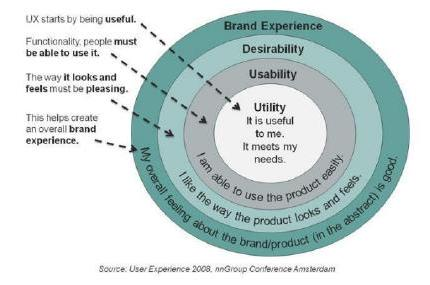
\includegraphics[width=0.6\linewidth]{images/2024_12_29_0d1d7b5551ea1b4b41bdg-02}
    
    \textbf{Wichtige Aspekte:}
    Benutzer und seine Ziele/Aufgaben, Kontext der Nutzung, Softwaresystem (inkl. UI)
\end{concept}

\begin{definition}{Usability-Dimensionen nach ISO 9241}
\begin{itemize}
    \item \textbf{Effektivität:}
    \begin{itemize}
        \item Der Benutzer kann alle Aufgaben vollständig erfüllen
        \item Gewünschte Genauigkeit wird erreicht
        \item Ziele werden im vorgegebenen Kontext erreicht
    \end{itemize}
    \end{itemize}

\begin{minipage}{0.5\linewidth}
    \begin{itemize}
    \item \textbf{Effizienz:} \\ Minimaler Aufwand für:
    \begin{itemize}
        \item Mentale Belastung
        \item Physische Anstrengung
        \item Zeitlicher Aufwand
        \item Ressourceneinsatz
    \end{itemize}
    \end{itemize}
\end{minipage}
\begin{minipage}{0.5\linewidth}
    \begin{itemize}
    \item \textbf{Zufriedenheit:}
    \begin{itemize}
        \item Minimum: Keine Verärgerung
        \item Standard: Zufriedenheit
        \item Optimal: Begeisterung
        \item Subjektive Nutzererfahrung
    \end{itemize}
\end{itemize}
\end{minipage}
\end{definition}

\begin{KR}{Usability-Evaluation durchführen}
\vspace{-2mm}\\
\begin{minipage}[t]{0.5\linewidth}
\begin{enumerate}[start=1]
    \item \textbf{Vorbereitung}
    \begin{itemize}
        \item Testziele definieren
        \item Testpersonen auswählen
        \item Testaufgaben erstellen
    \end{itemize}
    \item \textbf{Durchführung}
    \begin{itemize}
        \item Beobachtung der Nutzer
        \item Protokollierung von \\Problemen
        \item Zeitmessung der Aufgaben
    \end{itemize}
\end{enumerate}
\end{minipage}
\begin{minipage}[t]{0.5\linewidth}
\begin{enumerate}[start=3]
    \item \textbf{Auswertung}
    \begin{itemize}
        \item Probleme klassifizieren
        \item Schweregrad bestimmen
        \item Verbesserungen vorschlagen
    \end{itemize}
    
    \item \textbf{Dokumentation}
    \begin{itemize}
        \item Ergebnisse zusammenfassen
        \item Empfehlungen formulieren
        \item Maßnahmen priorisieren
    \end{itemize}
\end{enumerate}
\end{minipage}
\end{KR}

\begin{theorem}{ISO 9241-110: Usability-Anforderungen}

\begin{minipage}[t]{0.58\linewidth}
\begin{itemize}
    \item \textbf{Aufgabenangemessenheit:}
    \begin{itemize}
        \item Funktionalität unterstützt \\ Arbeitsaufgaben
        \item Keine unnötige Komplexität
    \end{itemize}
    
    \item \textbf{Selbstbeschreibungsfähigkeit:}
    \begin{itemize}
        \item Verständliche Benutzerführung
        \item Klare Statusanzeigen
    \end{itemize}
    
    \item \textbf{Steuerbarkeit:}
    \begin{itemize}
        \item Benutzer kontrolliert Ablauf
        \item Geschwindigkeit anpassbar
    \end{itemize}
    
    \item \textbf{Erwartungskonformität:}
    \begin{itemize}
        \item Konsistentes Verhalten
        \item Bekannte Konventionen
    \end{itemize}
\end{itemize}
\end{minipage}
\begin{minipage}[t]{0.4\linewidth}
\begin{itemize}    
    \item \textbf{Fehlertoleranz:}
    \begin{itemize}
        \item Fehler vermeiden
        \item Fehlerkorrektur \\ ermöglichen
    \end{itemize}
    
    \item \textbf{Individualisierbarkeit:}
    \begin{itemize}
        \item Anpassung an \\ Benutzergruppen
        \item Flexible Nutzung
    \end{itemize}
    
    \item \textbf{Lernförderlichkeit:}
    \begin{itemize}
        \item Einfacher Einstieg
        \item Unterstützung beim \\ Lernen
    \end{itemize}
\end{itemize}
\end{minipage}
\end{theorem}

\subsection{User-Centered Design (UCD)}

\begin{concept}{UCD Prozess}

\begin{minipage}{0.4\linewidth}
Ein iterativer Prozess zur nutzerzentrierten \\ Entwicklung, der die Bedürfnisse, Wünsche und Einschränkungen 
der Benutzer in jeder Phase des Design-Prozesses berücksichtigt.

\textbf{Hauptziele:}
\begin{itemize}
    \item Benutzerfreundlichkeit
    \item Effektive Nutzung
    \item Hohe Akzeptanz
\end{itemize}
\end{minipage}
\begin{minipage}{0.6\linewidth}
    \vspace{-5mm}
    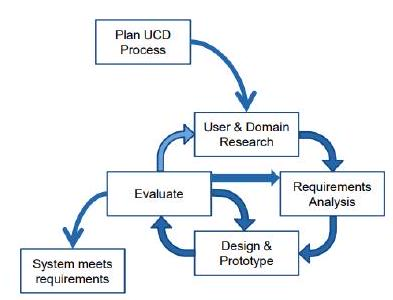
\includegraphics[width=\linewidth]{images/2024_12_29_0d1d7b5551ea1b4b41bdg-03}
\end{minipage}
\end{concept}

\begin{corollary}{Wichtige Artefakte}
\begin{itemize}
    \item Personas: Repräsentative Nutzerprofile
    \item Usage-Szenarien: Konkrete Anwendungsfälle
    \item Mentales Modell: Nutzerverständnis
    \item Domänenmodell: Fachliches Verständnis
    \item Service Blueprint: Geschäftsprozessmodell
    \item Stakeholder Map: Beteiligte und Betroffene
    \item UI-Artefakte: Skizzen, Wireframes, Designs
\end{itemize}
\end{corollary}

\begin{example2}{Stakeholder Map}\\
Zeigt die wichtigsten Stakeholder im Umfeld der Problemdomäne.\\
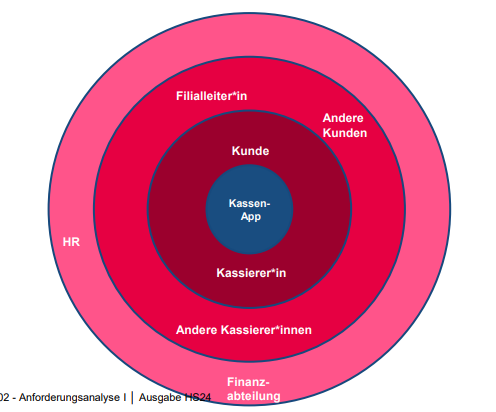
\includegraphics[width=0.8\linewidth]{images/stakeholdermap.png}
\end{example2}



\begin{theorem}{UCD Prozess-Phasen}\\
\textbf{1. User \& Domain Research} (see KR)

\textbf{2. Requirements Analysis} (see KR)

\begin{minipage}[t]{0.5\linewidth}
\textbf{3. Design \& Prototype}
\begin{itemize}
    \item Interaktionskonzept entwickeln
    \item Wireframes erstellen
    \item Prototypen bauen
    \item Design iterativ verbessern
\end{itemize}
\end{minipage}
\begin{minipage}[t]{0.5\linewidth}
\textbf{4. Evaluate}
\begin{itemize}
    \item Mit Benutzern testen
    \item Feedback sammeln
    \item Probleme identifizieren
    \item Verbesserungen einarbeiten
\end{itemize}
\end{minipage}
\end{theorem}

\begin{KR}{User \& Domain Research}
\begin{enumerate}
    \item \textbf{Zielgruppe identifizieren}
    \begin{itemize}
        \item Wer sind die Benutzer?
        \item Was sind ihre Aufgaben/Ziele?
        \item Wie sieht ihre Arbeitsumgebung aus?
        \item Welche Sprache/Begriffe verwenden sie?
    \end{itemize}
\end{enumerate}

\begin{minipage}[t]{0.5\linewidth}
\begin{enumerate}[start=2]
    \item \textbf{Daten sammeln durch}
    \begin{itemize}
        \item Contextual Inquiry
        \item Interviews
        \item Beobachtung
        \item Fokusgruppen
        \item Nutzungsauswertung
    \end{itemize}
\end{enumerate}
\end{minipage}
\begin{minipage}[t]{0.5\linewidth}
\begin{enumerate}[start=3]
    \item \textbf{Ergebnisse dokumentieren in}
    \begin{itemize}
        \item Personas
        \item Usage-Szenarien
        \item Mentales Modell
    \end{itemize}
\end{enumerate}
\end{minipage}
\end{KR}

\begin{KR}{UCD Artefakte erstellen}

\begin{minipage}[t]{0.45\linewidth}
\textbf{1. Personas}
\begin{itemize}
    \item Daten aus User Research\\ sammeln
    \item Gemeinsame Merkmale \\identifizieren
    \item Repräsentative Person \\definieren
    \item Details ausarbeiten:
    \begin{itemize}
        \item Demografische Daten
        \item Ziele und Motivation
        \item Fähigkeiten/Kenntnisse
        \item Frustrationspunkte
    \end{itemize}
\end{itemize}
\end{minipage}
\begin{minipage}[t]{0.5\linewidth}
\textbf{2. Usage-Szenarien}
\begin{itemize}
    \item Kontext beschreiben
    \item Akteure identifizieren
    \item Ablauf definieren
    \item Probleme/Lösungen darstellen
\end{itemize}

\textbf{3. Mentales Modell}
\begin{itemize}
    \item Nutzerverständnis\\ dokumentieren
    \item Konzepte und Beziehungen \\visualisieren
    \item Mit Fachmodell abgleichen
\end{itemize}
\end{minipage}
\end{KR}

\begin{example2}{Usage-Szenario: Online-Banking}\\
\textbf{Kontext:} Sarah möchte eine Überweisung tätigen

\textbf{Aktuelles Szenario:}
Sarah loggt sich in ihr Online-Banking ein. Sie sucht nach der letzten Überweisung an ihren Vermieter, um die Kontodetails zu finden. Nach mehreren Klicks findet sie die Information und kopiert die IBAN. Sie öffnet das Überweisungsformular und fügt die Daten ein. Beim Absenden erscheint eine Fehlermeldung, weil sie vergessen hat, den Verwendungszweck einzutragen.

\textbf{Probleme:}
\begin{itemize}
    \item Umständliche Suche nach Kontodetails
    \item Fehleranfällige manuelle Dateneingabe
    \item Späte Validierung der Eingaben
\end{itemize}

\textbf{Verbessertes Szenario:}
Sarah wählt aus einer Liste ihrer häufigen Empfänger ihren Vermieter aus. Das System füllt automatisch alle bekannten Daten ein. Fehlende Pflichtfelder sind deutlich markiert. Sarah ergänzt den Verwendungszweck und sendet die Überweisung ab.
\end{example2}

\begin{remark}
    Weitere Beispiele z.B. Persona erstellen auf nächster Seite
\end{remark}

\begin{example2}{Persona erstellen}\\
\textbf{Aufgabe:} Erstellen Sie eine Persona für ein Online-Banking-System.

\textbf{Lösung:} 
\textbf{Sarah Schmidt, 34, Projektmanagerin}
\begin{itemize}
    \item \textbf{Hintergrund:}
    \begin{itemize}
        \item Arbeitet Vollzeit in IT-Firma
        \item Technik-affin, aber keine Expertin
        \item Nutzt Smartphone für die meisten Aufgaben
    \end{itemize}
    \item \textbf{Ziele:}
    \begin{itemize}
        \item Schnelle Überweisungen zwischen Konten
        \item Überblick über Ausgaben
        \item Sichere Authentifizierung
    \end{itemize}
    \item \textbf{Frustrationen:}
    \begin{itemize}
        \item Komplexe Menüführung
        \item Lange Ladezeiten
        \item Mehrfache Login-Prozesse
    \end{itemize}
\end{itemize}
\end{example2}

\begin{example2}{Persona für E-Learning-System}\\
\textbf{Thomas Weber, 19, Informatik-Student}

\textbf{Hintergrund:}
\begin{itemize}
    \item Erstsemester-Student
    \item Arbeitet nebenbei 10h/Woche
    \item Pendelt zur Universität (1h pro Weg)
\end{itemize}

\textbf{Technische Fähigkeiten:}
\begin{itemize}
    \item Versiert im Umgang mit Computern
    \item Nutzt hauptsächlich Smartphone für Online-Aktivitäten
    \item Kennt gängige Learning-Management-Systeme
\end{itemize}

\textbf{Ziele:}
\begin{itemize}
    \item Effizientes Lernen trotz Zeitdruck
    \item Flexible Zugriffsmöglichkeiten auf Lernmaterialien
    \item Gute Prüfungsvorbereitung
\end{itemize}

\textbf{Frustrationen:}
\begin{itemize}
    \item Unübersichtliche Kursstrukturen
    \item Fehlende Mobile-Optimierung
    \item Schwierige Navigation zwischen Materialien
\end{itemize}
\end{example2}

\subsection{Requirements Engineering}

\begin{definition}{Requirements (Anforderungen)}
\begin{itemize}
    \item Leistungsfähigkeiten oder Eigenschaften
    \item Explizit oder implizit
    \item Müssen mit allen Stakeholdern erarbeitet werden
    \item Entwickeln sich während des Projekts
\end{itemize}
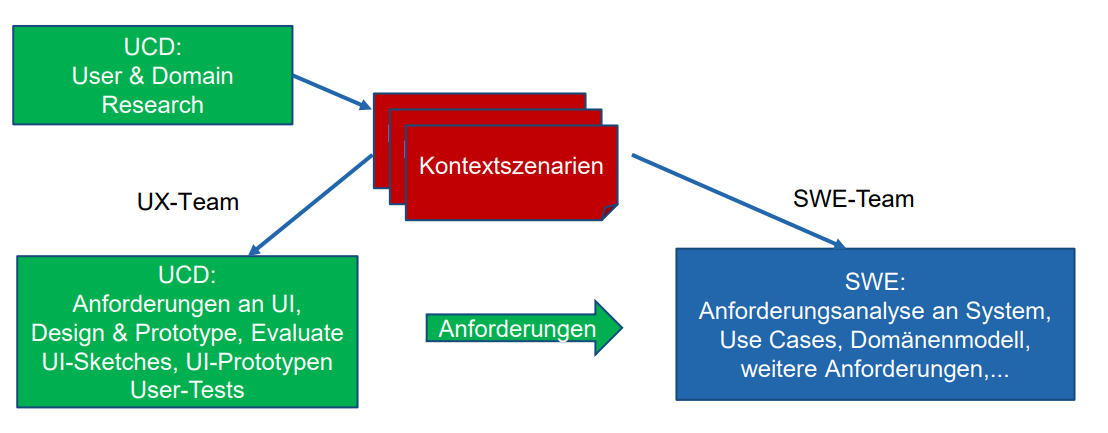
\includegraphics[width=\linewidth]{images/user_anforderungen.png}

\textbf{Charakteristiken:}
\begin{itemize}
    \item Können explizit oder implizit sein
    \item Sind fast nie im Vorneherein vollständig bekannt
    \item Müssen mit allen Stakeholdern erarbeitet werden
    \item Entwickeln sich während des Projekts
    \item Müssen verifizierbar und messbar sein
\end{itemize}

\textbf{Herkunft:}
\begin{itemize}
    \item Benutzer (Ziele, Bedürfnisse, Kontext)
    \item Weitere Stakeholder (Management, IT, etc.)
    \item Regulatorien, Gesetze, Normen
\end{itemize}
\end{definition}





\begin{concept}{Arten von Anforderungen}\\
\textbf{Funktionale Anforderungen:}
\begin{itemize}
    \item Beschreiben, WAS das System tun soll
    \item Werden in Use Cases dokumentiert
    \item Müssen konkret und testbar sein
\end{itemize}

\textbf{Nicht-funktionale Anforderungen (ISO 25010):}
\begin{itemize}
    \item Performance Efficiency
    \begin{itemize}
        \item Time Behaviour
        \item Resource Utilization
        \item Capacity
    \end{itemize}
    \item Compatibility
    \begin{itemize}
        \item Co-existence
        \item Interoperability
    \end{itemize}
    \item Usability (siehe oben)
    \item Reliability
    \begin{itemize}
        \item Maturity
        \item Availability
        \item Fault Tolerance
        \item Recoverability
    \end{itemize}
    \item Security
    \item Maintainability
    \item Portability
\end{itemize}

\textbf{Randbedingungen:}
\begin{itemize}
    \item Technische Einschränkungen
    \item Rechtliche Vorgaben
    \item Budgetäre Grenzen
    \item Zeitliche Limitationen
\end{itemize}
\end{concept}

\begin{KR}{Requirements Analysis}
    \begin{itemize}
        \item Benutzeranforderungen ableiten
        \item Kontextszenarien erstellen
        \item UI-Skizzen entwickeln
        \item Use Cases definieren
    \end{itemize}
    \vspace{2mm}

    \begin{minipage}[t]{0.45\linewidth}
    \textbf{Stakeholder identifizieren}
    \begin{itemize}
        \item Benutzer
        \item Auftraggeber
        \item Weitere Interessengruppen
    \end{itemize}
    
    \textbf{Anforderungsquellen \\ analysieren}
    \begin{itemize}
        \item Interviews und Workshops
        \item Existierende Dokumente
        \item Beobachtung der \\Arbeitsabläufe
    \end{itemize}
    \end{minipage}
    \begin{minipage}[t]{0.55\linewidth}    
    \textbf{Anforderungen dokumentieren}
    \begin{itemize}
        \item Funktionale Anforderungen \\ (Use Cases)
        \item Nicht-funktionale Anforderungen
        \item Randbedingungen
    \end{itemize}
    
    \textbf{Anforderungen validieren}
    \begin{itemize}
        \item Review mit Stakeholdern
        \item Priorisierung
        \item Machbarkeitsanalyse
    \end{itemize}
    \end{minipage}
\end{KR}

\begin{example2}{Anforderungsanalyse: Onlineshop}\\
\textbf{Ausgangssituation:}
Ein traditioneller Buchladen möchte einen Onlineshop entwickeln.

\textbf{Funktionale Anforderungen:}
\begin{itemize}
    \item Produktkatalog durchsuchen
    \item Warenkorb verwalten
    \item Bestellung aufgeben
    \item Kundenkonto verwalten
\end{itemize}

\textbf{Nicht-funktionale Anforderungen:}
\begin{itemize}
    \item Performance:
    \begin{itemize}
        \item Seitenaufbau < 2 Sekunden
        \item Suche < 1 Sekunde
    \end{itemize}
    \item Sicherheit:
    \begin{itemize}
        \item HTTPS-Verschlüsselung
        \item Zwei-Faktor-Authentifizierung
    \end{itemize}
    \item Usability:
    \begin{itemize}
        \item Responsive Design
        \item Max. 3 Klicks zur Bestellung
    \end{itemize}
\end{itemize}

\textbf{Randbedingungen:}
\begin{itemize}
    \item DSGVO-Konformität
    \item Integration mit bestehendem ERP
    \item Budget: 100.000 EUR
    \item Launch in 6 Monaten
\end{itemize}
\end{example2}

\columnbreak



\subsection{Use Cases}

\begin{definition}{Use Case (Anwendungsfall)}\\
Ein Use Case beschreibt eine konkrete Interaktion zwischen Akteur und System mit folgenden Eigenschaften:

\textbf{Grundprinzipien:}
\begin{itemize}
    \item Aus Sicht des Akteurs beschrieben
    \item Aktiv formuliert (Verb + Objekt)
    \item Konkreter Nutzen für Akteur
    \item Mehr als eine einzelne Interaktion
    \item Essentieller Stil (Logik statt Implementierung)
\end{itemize}

\textbf{Qualitätskriterien:}
\begin{itemize}
    \item Boss-Test: Sinnvolle Arbeitseinheit
    \item EBP-Test: Elementary Business Process
    \item Size-Test: Mehrere Interaktionen
\end{itemize}
\end{definition}

\begin{KR}{Use Case Erstellung}\\
Schritte zur Erstellung eines vollständigen Use Cases:
\begin{enumerate}
    \item \textbf{Identifikation:} siehe \textcolor{green}{\textbf{Use Case Identifikation}}
    \item \textbf{Dokumentation:}
    \begin{itemize}
        \item Brief/Casual für erste Analyse
        \item Fully-dressed für wichtige Use Cases
        \item Standardablauf und Erweiterungen
    \end{itemize}
    \item \textbf{Review:}
    \begin{itemize}
        \item Mit Stakeholdern abstimmen
        \item Auf Vollständigkeit prüfen
        \item Konsistenz sicherstellen
    \end{itemize}
\end{enumerate}
\end{KR}

\begin{theorem}{Use Case Identifikation}
\begin{enumerate}
    \item \textbf{Systemgrenzen definieren}
    \begin{itemize}
        \item Was gehört zum System?
        \item Was ist externe Umgebung?
    \end{itemize}
    \item \textbf{Akteure identifizieren}
    \item \textbf{Ziele ermitteln}
    \begin{itemize}
        \item Geschäftsziele
        \item Benutzerziele
        \item Systemziele
    \end{itemize}
\end{enumerate}
\end{theorem}

\begin{corollary}{Akteure in Use Cases}
\begin{itemize}
    \item \textbf{Primärakteur:} Initiiert den Use Case, erhält Hauptnutzen
    \item \textbf{Unterstützender Akteur:} Hilft bei der Durchführung
    \item \textbf{Offstage-Akteur:} Indirekt beteiligter Stakeholder
\end{itemize}
\end{corollary}

\begin{concept}{Use Case Beziehungen}\\
\textbf{Include-Beziehung:}
\begin{itemize}
    \item Ein UC schließt einen anderen UC ein
    \item Wiederverwendung von Funktionalität
    \item Obligatorische Beziehung
\end{itemize}

\textbf{Extend-Beziehung:}
\begin{itemize}
    \item Optionale Erweiterung eines UC
    \item Unter bestimmten Bedingungen
    \item Ursprünglicher UC bleibt unverändert
\end{itemize}

\textbf{Generalisierung:}
\begin{itemize}
    \item Spezialisierung von Akteuren/UCs
    \item Vererbung von Eigenschaften
    \item "ist-ein"-Beziehung
\end{itemize}
\end{concept}

\begin{concept}{Use Case Granularität}
\begin{enumerate}
    \item \textbf{Brief Use Case}
    \begin{itemize}
        \item Kurze Zusammenfassung
        \item Hauptablauf skizzieren
        \item Keine Details zu Varianten
    \end{itemize}
    \item \textbf{Casual Use Case}
    \begin{itemize}
        \item Mehrere Absätze
        \item Hauptvarianten beschreiben
        \item Informeller Stil
    \end{itemize}
    \item \textbf{Fully-dressed Use Case}
    \begin{itemize}
        \item Vollständige Struktur
        \item Alle Varianten
        \item Vor- und Nachbedingungen
        \item Garantien definieren
    \end{itemize}
\end{enumerate}
\end{concept}

\begin{KR}{Fully-dressed Use Case erstellen}

\begin{minipage}[t]{0.55\linewidth}
\textbf{1. Grundinformationen}
\begin{itemize}
    \item Aussagekräftiger Name (aktiv)
    \item Umfang (Scope)
    \item Ebene (Level)
    \item Primärakteur
\end{itemize}

\textbf{2. Stakeholder und Interessen}
\begin{itemize}
    \item Alle beteiligten Parteien
    \item Deren spezifische Interessen
\end{itemize}

\textbf{3. Vor- und Nachbedingungen}
\begin{itemize}
    \item Was muss vorher erfüllt sein?
    \item Was ist nachher garantiert?
\end{itemize}
\end{minipage}
\begin{minipage}[t]{0.45\linewidth}
\textbf{4. Standardablauf}
\begin{itemize}
    \item Nummerierte Schritte
    \item Akteur-System-Interaktion
    \item Klare Erfolgskriterien
\end{itemize}

\textbf{5. Erweiterungen}
\begin{itemize}
    \item Alternative Abläufe
    \item Fehlerszenarien
    \item Verzweigungen
\end{itemize}
\end{minipage}
\end{KR}

\begin{example2}{Brief Use Case}
\textbf{Verkauf abwickeln}

Kunde kommt mit Waren zur Kasse. Kassier erfasst alle Produkte. System berechnet Gesamtbetrag. Kassier nimmt Zahlung entgegen und gibt ggf. Wechselgeld. System druckt Beleg.
\end{example2}

%TODO: Add casual use case?

\begin{example2}{Casual Use Case}
\textbf{UC: Verkauf abwickeln}
Der Umfang des Use Cases ist das Kassensystem. Der Primärakteur ist der Kassier. 
Der Stakeholder ist der Kunde, der eine schnelle Abwicklung wünscht, und das Geschäft, das eine korrekte Abrechnung benötigt. 
Die Vorbedingung ist, dass die Kasse geöffnet ist.
\vspace{2mm}\\
Der Standardablauf ist wie folgt:
Kassier startet neuen Verkauf und System initialisiert neue Transaktion. Kassier erfasst Produkte und System zeigt Zwischensumme. 
Kassier schliesst Verkauf ab und System zeigt Gesamtbetrag. Kunde bezahlt und System druckt Beleg.
\end{example2}


\begin{example2}{Fully-dressed Use Case}
\textbf{UC: Verkauf abwickeln}
\begin{itemize}
    \item \textbf{Umfang:} Kassensystem
    \item \textbf{Primärakteur:} Kassier
    \item \textbf{Stakeholder:} Kunde (schnelle Abwicklung), Geschäft (korrekte Abrechnung)
    \item \textbf{Vorbedingung:} Kasse ist geöffnet
    \item \textbf{Standardablauf:}
    \begin{enumerate}
        \item Kassier startet neuen Verkauf
        \item System initialisiert neue Transaktion
        \item Kassier erfasst Produkte
        \item System zeigt Zwischensumme
        \item Kassier schliesst Verkauf ab
        \item System zeigt Gesamtbetrag
        \item Kunde bezahlt
        \item System druckt Beleg
    \end{enumerate}
\end{itemize}
\end{example2}

\begin{example2}{Fully-dressed Use Case}
\textbf{Aufgabe:} Erstellen Sie einen fully-dressed Use Case für ein Online-Bibliothekssystem. Fokus: "Buch ausleihen"

\textbf{Lösung:}
\begin{itemize}
    \item \textbf{Umfang:} Online-Bibliothekssystem
    \item \textbf{Primärakteur:} Bibliotheksnutzer
    \item \textbf{Stakeholder:} 
    \begin{itemize}
        \item Bibliotheksnutzer: Möchte Buch einfach ausleihen
        \item Bibliothek: Korrekte Erfassung der Ausleihe
    \end{itemize}
    \item \textbf{Vorbedingung:} Nutzer ist eingeloggt
    \item \textbf{Standardablauf:}
    \begin{enumerate}
        \item Nutzer sucht Buch
        \item System zeigt Verfügbarkeit
        \item Nutzer wählt Ausleihe
        \item System prüft Ausleihberechtigung
        \item System registriert Ausleihe
        \item System zeigt Bestätigung
    \end{enumerate}
    \item \textbf{Erweiterungen:}
    \begin{itemize}
        \item 2a: Buch nicht verfügbar
        \item 4a: Keine Ausleihberechtigung
    \end{itemize}
\end{itemize}
\end{example2}

\begin{example2}{Typische Prüfungsaufgabe: Use Case Analyse}\\
\textbf{Aufgabe:} Analysieren Sie den folgenden Use Case und identifizieren Sie mögliche Probleme:

\textbf{Use Case:} "Der Benutzer loggt sich ein und das System zeigt die Startseite. Er klickt auf den Button und die Daten werden in der Datenbank gespeichert."

\textbf{Probleme:}
\begin{itemize}
    \item Zu technisch/implementierungsnah
    \item Fehlende Akteurperspektive
    \item Unklarer Nutzen/Ziel
    \item Fehlende Alternativszenarien
    \item Keine Fehlerbehandlung
\end{itemize}

\textbf{Verbesserter Use Case:}
"Der Kunde möchte seine Bestelldaten speichern. Er bestätigt die Eingaben und erhält eine Bestätigung über die erfolgreiche Speicherung."
\end{example2}

\begin{example2}{Prüfungsaufgabe: Use Case Analyse}\\
\textbf{Aufgabe:} Analysieren Sie folgenden Use Case und verbessern Sie ihn.

\textbf{Ursprünglicher Use Case:}
"Der User loggt sich ein. Das System überprüft seine Credentials in der Datenbank. 
Bei erfolgreicher Validierung wird die Startseite angezeigt. Der User klickt auf 'Profil bearbeiten' 
und das System speichert die Änderungen in der Datenbank."

\textbf{Probleme:}
\begin{itemize}
    \item Technische Implementierungsdetails
    \item Fehlende Akteurperspektive
    \item Keine Alternativen/Fehlerbehandlung
    \item Unklarer Nutzen/Ziel
\end{itemize}

\textbf{Verbesserter Use Case:}
"Profilinformationen aktualisieren"
\begin{itemize}
    \item \textbf{Primärakteur:} Registrierter Benutzer
    \item \textbf{Vorbedingung:} Benutzer ist authentifiziert
    \item \textbf{Standardablauf:}
    \begin{enumerate}
        \item Benutzer wählt Profilbearbeitung
        \item System zeigt aktuelle Profildaten
        \item Benutzer ändert gewünschte Informationen
        \item System prüft Änderungen
        \item System bestätigt erfolgreiche Aktualisierung
    \end{enumerate}
    \item \textbf{Erweiterungen:}
    \begin{itemize}
        \item 4a: Ungültige Eingaben
        \item 4b: Verbindungsfehler
    \end{itemize}
\end{itemize}
\end{example2}


\columnbreak

\subsection{System Sequence Diagrams}

\begin{definition}{Systemsequenzdiagramm (SSD)}\\
Formalisierte Darstellung der System-Interaktionen:

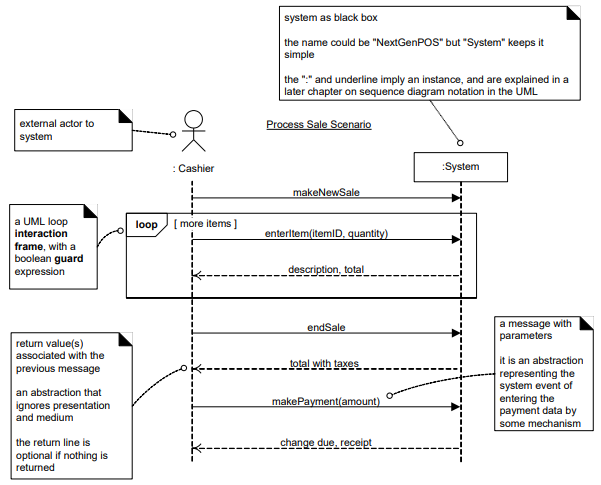
\includegraphics[width=\linewidth]{images/ssd.png}
\end{definition}

\begin{concept}{System Sequence Diagram}\\
Ein SSD visualisiert die Interaktion zwischen Akteur und System auf einer höheren Abstraktionsebene:

\textbf{Hauptmerkmale:}
\begin{itemize}
    \item Zeigt Input/Output-Events
    \item Identifiziert Systemoperationen
    \item Bildet Basis für API-Design
    \item Abstrahiert von UI-Details
\end{itemize}

\textbf{Notationselemente:}
\begin{itemize}
    \item Akteur und System als Lebenslinien
    \item Methodenaufrufe als durchgezogene Pfeile
    \item Rückgabewerte als gestrichelte Pfeile
    \item Parameter für benötigte Informationen
\end{itemize}
\end{concept}

\begin{KR}{System Sequence Diagram erstellen}\\
\textbf{1. Vorbereitung}
\begin{itemize}
    \item Use Case als Grundlage wählen
    \item Standardablauf identifizieren
    \item Akteur und System festlegen
\end{itemize}

\textbf{2. Methodenaufrufe definieren}
\begin{itemize}
    \item Aussagekräftige Namen wählen
    \item Notwendige Parameter bestimmen
    \item Rückgabewerte festlegen
\end{itemize}

\textbf{3. Zeitliche Abfolge}
\begin{itemize}
    \item Sequenz der Aufrufe modellieren
    \item Abhängigkeiten beachten
    \item Kontrollstrukturen einbauen (alt, loop, etc.)
\end{itemize}

\textbf{4. Externe Systeme}
\begin{itemize}
    \item Bei Bedarf weitere Akteure einbinden
    \item Schnittstellen definieren
    \item Kommunikationsfluss darstellen
\end{itemize}
\end{KR}

\begin{KR}{Systemoperationen definieren}\\
\textbf{Namenskonventionen:}
\begin{itemize}
    \item Verben für Aktionen
    \item Substantive für Entitäten
    \item Präzise, aber nicht technisch
\end{itemize}

\textbf{Parameter:}
\begin{itemize}
    \item Nur notwendige Information
    \item Domänenorientierte Typen
    \item Sinnvolle Standardwerte
\end{itemize}

\textbf{Rückgabewerte:}
\begin{itemize}
    \item Eindeutige Bestätigungen
    \item Relevante Geschäftsobjekte
    \item Fehlerindikationen
\end{itemize}

\textbf{Beispiele guter Operationen:}
\begin{lstlisting}[language=Java, style=base]
// Gut - klar und domaenenorientiert
createOrder(customer: CustomerId): OrderId
addOrderItem(orderId: OrderId, 
            product: ProductId, 
            quantity: int)

// Schlecht - zu technisch/implementierungsnah
insertIntoOrderTable(customerData: Map)
updateOrderItemList(items: ArrayList)
\end{lstlisting}
\end{KR}

\begin{KR}{Contracts für Systemoperationen}\\
Ein Contract definiert die Vor- und Nachbedingungen einer Systemoperation:

\textbf{1. Struktur}
\begin{itemize}
    \item Name und Parameter
    \item Querverweis zum Use Case
    \item Vorbedingungen
    \item Nachbedingungen
\end{itemize}

\textbf{2. Vorbedingungen}
\begin{itemize}
    \item Systemzustand vor Aufruf
    \item Notwendige Initialisierungen
    \item Gültige Parameter
\end{itemize}

\textbf{3. Nachbedingungen}
\begin{itemize}
    \item Erstellte/gelöschte Instanzen
    \item Geänderte Attribute
    \item Neue/gelöschte Assoziationen
\end{itemize}
\end{KR}

\begin{example2}{Contract für enterItem()}\\
\textbf{Operation:} enterItem(itemId: ItemID, quantity: int)

\textbf{Querverweis:} UC "Process Sale"

\textbf{Vorbedingungen:}
\begin{itemize}
    \item Verkauf ist gestartet
    \item ItemID existiert im System
\end{itemize}

\textbf{Nachbedingungen:}
\begin{itemize}
    \item SalesLineItem-Instanz wurde erstellt
    \item Verknüpfung mit aktueller Sale-Instanz
    \item quantity wurde gesetzt
    \item Verknüpfung mit ProductDescription
\end{itemize}
\end{example2}

\columnbreak

\begin{example2}{SSD Übungsaufgabe}\\
\textbf{Aufgabe:} Erstellen Sie ein Systemsequenzdiagramm für den Use Case 'Geld abheben' an einem Bankautomaten.

\textbf{Wichtige Aspekte:}
\begin{itemize}
    \item Kartenvalidierung
    \item PIN-Eingabe
    \item Betragseingabe
    \item Kontostandsprüfung
    \item Geldausgabe
    \item Belegdruck
\end{itemize}

\textbf{Essentielle Systemoperationen:}
\begin{itemize}
    \item validateCard(cardNumber)
    \item checkPIN(pin)
    \item withdrawMoney(amount)
    \item printReceipt()
\end{itemize}

\textbf{Sequenzdiagramm:} %TODO: add SSD graphic
\textcolor{pink}{\textbf{TO BE ADDED}}
\end{example2}

\columnbreak

\begin{example2}{SSD: Online-Banking Überweisung}\\
\textbf{Use Case:} Überweisung durchführen

\textbf{Systemoperationen:}
\begin{lstlisting}[language=Java, style=base]
// Kontostand pruefen
checkBalance(): Money

// Ueberweisung initiieren
initiateTransfer(recipient: String, 
                iban: String, 
                amount: Money, 
                purpose: String): TransferId

// TAN anfordern
requestTAN(transferId: TransferId): void

// Ueberweisung bestaetigen
confirmTransfer(transferId: TransferId, 
               tan: String): Boolean
\end{lstlisting}

\textbf{Wichtige Aspekte:}
\begin{itemize}
    \item Validierung vor Ausführung
    \item Zweistufige Bestätigung
    \item Klare Rückmeldungen
    \item Fehlerbehandlung
\end{itemize}

\textbf{Sequenzdiagramm:} %TODO: add SSD graphic
\textcolor{pink}{\textbf{TO BE ADDED}}
\end{example2}

\columnbreak

\begin{example2}{SSD: Typische Prüfungsaufgabe}\\
\textbf{Aufgabe:} Erstellen Sie ein SSD für den Use Case "Produkt bestellen" in einem Webshop.

\textbf{Analyse:}
\begin{itemize}
    \item Identifiziere Hauptaktionen:
    \begin{itemize}
        \item Warenkorb verwalten
        \item Bestellung aufgeben
        \item Zahlung durchführen
    \end{itemize}
    
    \item Definiere Systemoperationen:
    \begin{itemize}
        \item addToCart(productId, quantity)
        \item showCart(): CartContents
        \item checkout(shippingAddress, paymentMethod)
        \item confirmOrder(): OrderId
    \end{itemize}
    
    \item Berücksichtige Rückgabewerte:
    \begin{itemize}
        \item Bestätigungen
        \item Zwischensummen
        \item Fehlermeldungen
    \end{itemize}
\end{itemize}

\textbf{Sequenzdiagramm:} %TODO: add SSD graphic
\textcolor{pink}{\textbf{TO BE ADDED}}
\end{example2}

\columnbreak

\begin{example2}{SSD: Integration mit externen Systemen}\\
\textbf{Use Case:} Kreditkartenzahlung durchführen

\textbf{Beteiligte Systeme:}
\begin{itemize}
    \item Verkaufssystem (SuD)
    \item Kreditkarten-Autorisierungssystem
    \item Buchhaltungssystem
\end{itemize}

\textbf{Systemoperationen:}
\begin{lstlisting}[language=Java, style=base]
// Request credit card approval
requestApproval(cardNum: String, 
               expiryDate: Date, 
               amount: Money): Boolean

// Post transaction to accounting
postTransaction(transactionData: TransactionData)
\end{lstlisting}

\textbf{Wichtige Aspekte:}
\begin{itemize}
    \item Asynchrone Kommunikation
    \item Fehlerbehandlung über mehrere Systeme
    \item Transaktionsmanagement
    \item Logging und Nachvollziehbarkeit
\end{itemize}

\textbf{Sequenzdiagramm:} %TODO: add SSD graphic
\textcolor{pink}{\textbf{TO BE ADDED}}
\end{example2}